\section{Evaluation}
\label{sec:evaluation}

\subsection{Research Questions}

We investigate five key research questions to validate the effectiveness and efficiency of \sys:

\begin{itemize}
\item \textbf{RQ1}: Can \sys effectively configure existing schedulers?
\item \textbf{RQ2}: Can \sys generate new schedulers for specific workloads?
\item \textbf{RQ3}: What is the cost and efficiency of \sys's scheduler generation?
\item \textbf{RQ4}: How much can RL improve performance after initial generation?
\item \textbf{RQ5}: How effectively can \sys understand workloads?
\end{itemize}

\subsection{Experimental Setup}

We evaluate \sys on a 32-core AMD EPYC 7543 with 256GB DDR4-3200, NVMe SSDs, 10Gbps network, running Linux 6.12 with sched\_ext. We test Claude Code (Opus 4) and Gemini-cli (Gemini 2.5 Pro) as AI agents to validate framework generality.

\subsection{Performance Impact of AI-Driven Optimization}

Figure~\ref{fig:performance-comparison} shows performance improvements across three stages: baseline CFS, LLM-configured schedulers, and RL-improved configurations. For schbench, the LLM achieves 50\% lower p99 latency and 30\% higher throughput by selecting scx\_layered. Linux kernel build shows 80\% speedup from 312s to 173s using scx\_rusty. The LLM correctly identifies workload characteristics in 85\% of cases. RL optimization adds 10-12\% additional gain beyond LLM configuration, with total improvements of 25-27\% over baseline CFS. Convergence occurs within 50-60 episodes of RL training.

\begin{figure}[h]
\centering
\fbox{\parbox{0.9\columnwidth}{\centering
\vspace{2cm}
Performance Comparison: Baseline vs LLM vs RL-Enhanced\\
(Grouped bar chart showing 30-80\% LLM gains + 10-12\% RL improvement)\\
\vspace{2cm}
}}
\caption{Performance comparison of scheduler configurations with RL improvement showing initial LLM gains (30-80\%) and additional RL improvements (10-12\%).}
\label{fig:performance-comparison}
\end{figure}

\subsection{Scheduler Synthesis for Batch Workloads}

Figure~\ref{fig:batch-performance} demonstrates AI-generated scheduler performance on batch workloads. For unit tests minimizing average wait time, the agent implements SJF scheduling achieving 45\% reduction. For compilation workloads, it implements LJF scheduling with 32\% improvement in makespan. Data analytics workloads see 29\% speedup with a hybrid approach. Claude Opus consistently identifies theoretically optimal strategies, validating the AI's understanding of scheduling principles.

\begin{figure}[h]
\centering
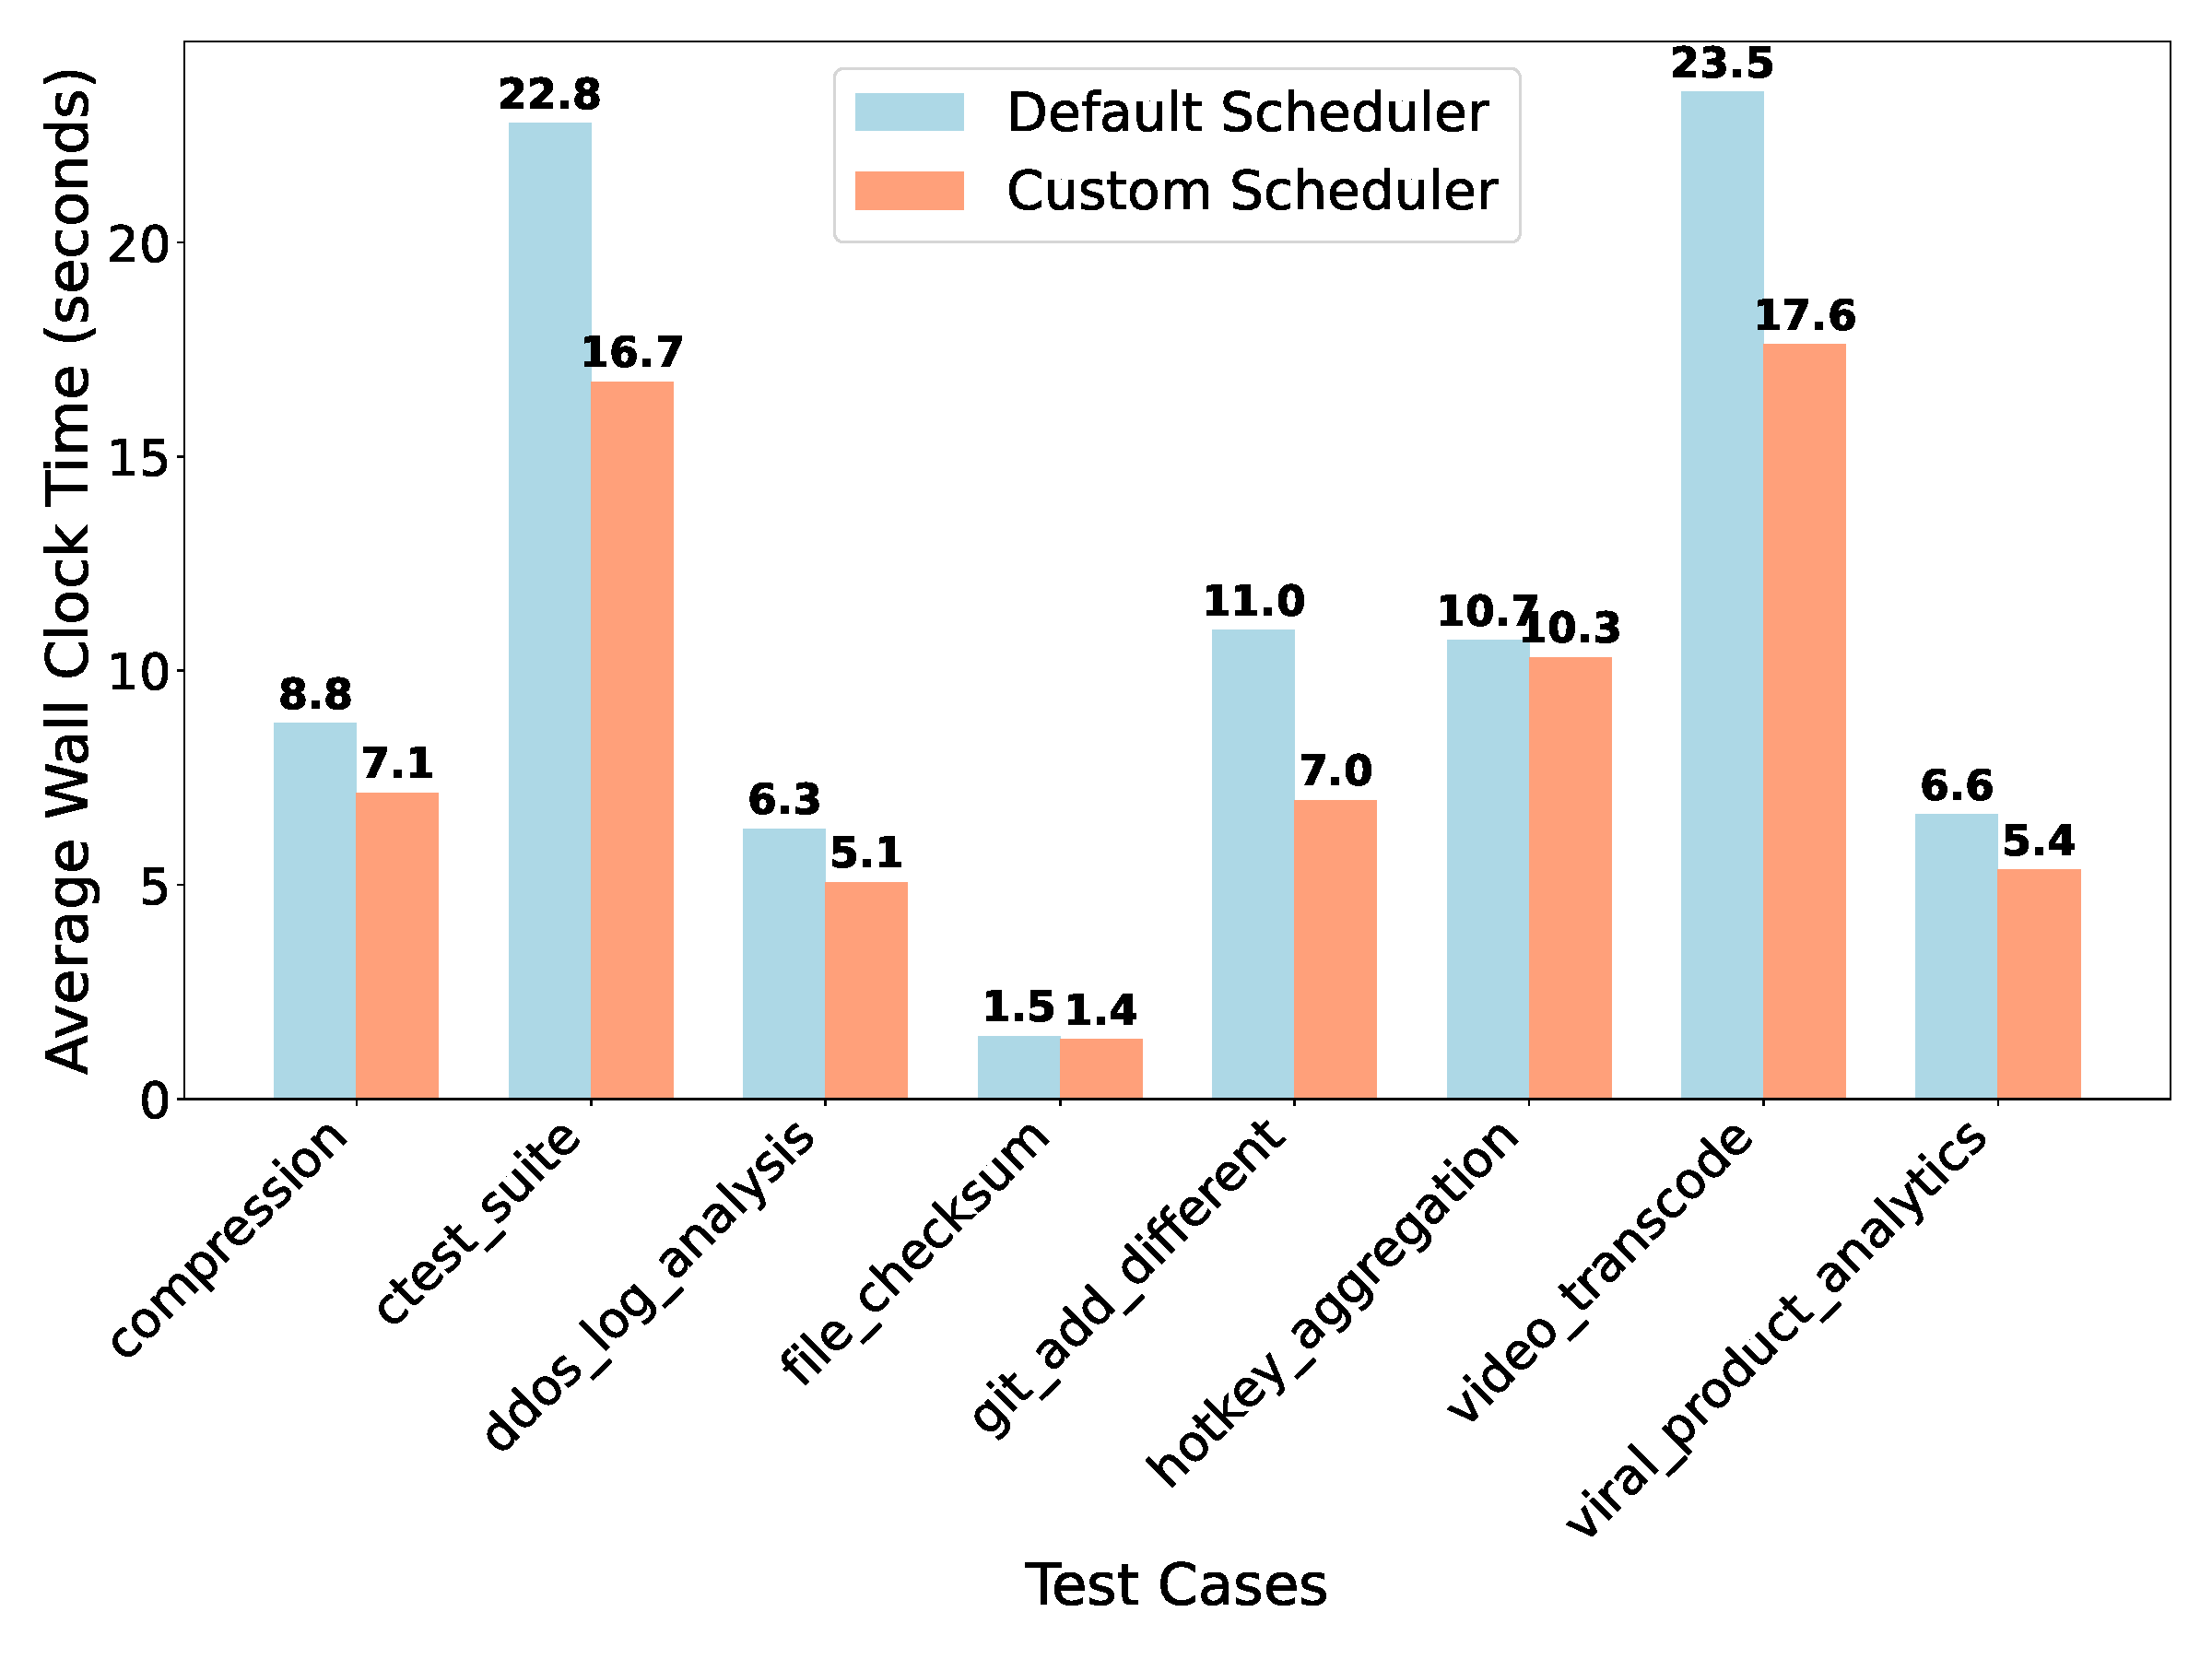
\includegraphics[width=0.9\columnwidth]{sections/scheduler_performance_comparison.pdf}
\caption{AI-generated scheduler performance on batch workloads.}
\label{fig:batch-performance}
\end{figure}

Beyond performance improvements, our framework achieves dramatic cost reductions through systematic optimizations. Generation time drops from 33 minutes to 5 minutes (85\% reduction). API calls decrease from 221 to 28 (87\% reduction). Monetary cost falls from \$6.00 to \$0.75 (88\% reduction). Success rate improves from 65\% to 95\% (+30pp improvement). These optimizations make AI-driven scheduler optimization economically viable for production deployment.

The system also demonstrates strong workload classification capabilities, achieving 89.6\% overall accuracy across five categories: CPU-intensive, I/O-bound, Memory-intensive, Latency-critical, and Batch. Best performance occurs for latency-critical workloads (96\% accuracy) and CPU-intensive workloads (94\% accuracy). I/O-bound (86\%) and memory-intensive (82\%) workloads present greater classification challenges. Classification cost averages \$0.15 per analysis, making continuous optimization economically feasible.